\documentclass[a4paper,10pt]{jsarticle}

% 数式
\usepackage{amsmath,amsfonts}
\usepackage{bm}
% 画像
\usepackage[dvipdfmx]{graphicx}
\usepackage{here}

\usepackage{listingsutf8,jlisting} %日本語のコメントアウトをする場合jlistingが必要
%ここからソースコードの表示に関する設定
\lstset{
  basicstyle={\ttfamily},
  identifierstyle={\small},
  commentstyle={\smallitshape},
  keywordstyle={\small\bfseries},
  ndkeywordstyle={\small},
  stringstyle={\small\ttfamily},
  frame={tb},
  breaklines=true,
  columns=[l]{fullflexible},
  numbers=left,
  xrightmargin=0zw,
  xleftmargin=3zw,
  numberstyle={\scriptsize},
  stepnumber=1,
  numbersep=1zw,
  lineskip=-0.5ex
}

\begin{document}

\title{ソフトウェア設計法レポート}
\author{坪井正太郎(101830245)}
\date{\today}
\maketitle
フリマアプリのユーザー情報、特にユーザー間での問い合わせについて考察した。
\section{既存のデータやオブジェクトの説明とその定義}
以下のようなユーザー情報をオブジェクトとして定義する。
このとき、このユーザーに対して問い合わせを行いたいときはメールアドレスを参照して、メールを送信する。
また、運営から重要なメッセージやものを送りたいときには、住所や電話番号から適切に選択して送信する必要がある。
\begin{figure}[H]
  \centering
  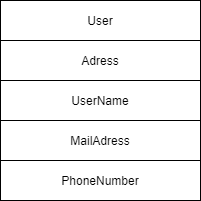
\includegraphics[width=\linewidth]{./01.drawio.png}
  \caption{既存のユーザーオブジェクト}
  \label{}
\end{figure}

\section{将来の変更とそれに強いオブジェクトの定義}
将来、メールアドレスではなく、web上のGUIクライアントによってメッセージをやりとりするように使用が変更される可能性がある。

オブジェクトには、問い合わせや通知に対応するメソッドを実装する。
そうして、以下のようなユーザー情報をオブジェクトとして定義する。
\begin{figure}[H]
  \centering
  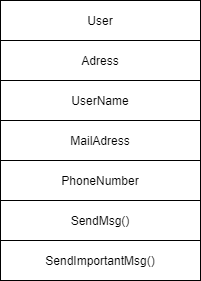
\includegraphics[width=\linewidth]{./02.drawio.png}
  \caption{変更に強いユーザーオブジェクト}
  \label{}
\end{figure}

\section{変更に強い理由}
問い合わせの発生するすべての部分でメールアドレスを参照する必要がなくなり、メソッド実装の変更のみで済むことになるため、変更に強いと言える。

\end{document}
